\chapter{\huge Integrazione Numerica}

\textit{In analisi numerica, l'integrazione numerica consiste in una serie di metodi che stimano il valore di un integrale definito, senza dover calcolare la primitiva della funzione integranda. In questa sezione si illustrano alcuni dei principali metodi deterministici e non.}

\section{Newton-Cotes}
Le regole di quadratura di Newton-Cotes sono formule che consistono nel valutare l'integrando in punti equispaziati dell'intervallo di integrazione.

Si assume che il valore di una funzione $f:[a,b]\in\mathbb{R}\rightarrow\mathbb{R}$ sia noto nei punti $x_i$, per $i=0,...,n$ tali che $$x_i=a+\left(\frac{b-a}{n}\right)i$$
La formula di Newton-Cotes di grado $n$ si ottiene interpolando $f$ nei punti $x_i$ con i polinomi della base di Lagrange, e integrando la polinomiale risultante, $L(x)$, nell'intervallo $[a,b]$.
$$ \int_a^b f(x) \,dx \approx \int_a^b L(x)\,dx = \int_a^b \bigl( \sum_{i=0}^n f(x_i)\, \ell_i(x) \bigr) \, dx = \sum_{i=0}^n f(x_i) \underbrace{\int_a^b \ell_i(x)\, dx}_{w_i} $$
dove gli $\ell_i(x)$ sono i polinomi di Lagrange così definiti
$$\ell_i(x):= \prod_{\begin{smallmatrix}0\le j\le n\\ j\neq i\end{smallmatrix}} \frac{x-x_j}{x_i-x_j}$$$$\ell_i(x_j)=\delta_{ij}$$
La formula di Newton-Cotes assume così la semplice forma di media dei valori $f(x_i)$ pesati sui coefficienti $w_i$ (indipendenti da $f$)
$$\int_a^b f(x) \,dx \approx \sum_{i=0}^n w_i\, f(x_i)$$
Si domostra che l'errore dell'interpolazione di $f$ con un polinomio è
$$E(x)=\frac{1}{(n+1)!}f^{(n+1)}(\xi(x))\prod_{i=0}^n(x-x_i)$$
per un certo $\xi\in[a,b]$ dipendente da $x$. Non avendo tuttavia alcuna informazione su come individuare il punto $\xi$ in genere si effettua solo una stima del limite superiore sull'errore $E(x)$ per $\xi$ tale che $f(\xi) = \underset{x\in[a,b]}{\max}f(x)$.

Al primo ordine dell'approssimazione Newton-Cotes la formula si riduce al cosidetto metodo dei ``trapezi'':
$$\int_a^b f(x) \,dx=\frac{b-a}{2}\left[ f(a)+f(b)\right] + \underbrace{\frac{1}{2}\int_a^b f''(\xi(x))(x-a)(x-b)}_{E_1}$$
mentre al secondo ordine non è altro che la regola di Simpson:
$$\int_a^b f(x) \,dx=\frac{b-a}{3}\left[f(a)+4f(\frac{a+b}{2})+f(b)\right] + \underbrace{\frac{1}{6}\int_a^b f'''(\xi(x))(x-a)(x-\frac{a+b}{2})(x-b)}_{E_2}$$

\section{Quadrature Gaussiane}
La regola di quadratura Gaussiana a $n$-punti è un metodo di integrazione numerica costruito in modo tale da fornire un risultato esatto per polinomi di grado inferiore a $2n$, attraverso una scelta appropriata di punti $x_i$ e pesi $w_i$, per $i=1,...,n$. Sul dominio di integrazione convenzionale $[-1,1]$ la regola è così formulata
$$\int_{-1}^1 f(x)\,dx \approx \sum_{i=1}^n w_i f(x_i)$$
L'accuratezza del risultato è tanto più grande quanto meglio $f$ è approssimata da un polinomio. Se tuttavia la funzione integranda può essere scritta come $f(x)=W(x)g(x)$, dove $g(x)$ è approssimativamente polinomiale e $W(x)$ è nota, allora esistono $w'_i$ tali che
$$\int_{-1}^1 f(x)\,dx = \int_{-1}^1 W(x) g(x)\,dx \approx \sum_{i=1}^n w_i' g(x_i)$$
$W(x)$ viene detta funzione peso, mentre i punti $x_i$ sono le radici di un polinomio appartenente alla classe dei polinomi ortogonali.

Nel caso considerato $W(x)=1$ ed i polinomi associati sono i polinomi ortogonali di Legendre $P_n(x)$. Il peso $i$-esimo associato al nodo Gaussiano $x_i$ è dato da
$$ w_i = \frac{2}{\left( 1-x_i^2 \right) [P'_n(x_i)]^2} \,\!$$
Analogamente alle regole di Newton-Cotes, l'errore teorico del metodo della quadratura Gaussiana è
$$E(x)=\frac{1}{n!}f^{(n)}(\xi(x))\prod_{i=1}^n(x-x_i)$$
che può tuttavia essere ridotto a
$$E(x)=\frac{1}{(2n)!}f^{(2n)}(\xi(x))\prod_{i=1}^n(x-x_i)^2$$
semplicemente considerando due volte ogni punto di interpolazione $x_i$.

Infine, se si vuole calcolare l'integrale su $[a,b]$ invece che sull'intervallo $[-1,1]$, si deve effettuare il cambio di variabile
$$\int_a^b f(x)\,dx = \frac{b-a}{2} \int_{-1}^1 f\left(\frac{b-a}{2}x + \frac{a+b}{2}\right)\,dx $$
ed applicando il metodo di Gauss si ottiene
$$\int_a^b f(x)\,dx \approx \frac{b-a}{2} \sum_{i=1}^n w_i f\left(\frac{b-a}{2}x_i + \frac{a+b}{2}\right)$$
I nodi ed i pesi per il polinomio di Legendre di quinto grado sono riportati in tabella:\\
\begin{center}
\scalebox{1.5}{
\begin{tabular}{|c|c|}
\hline
$x_i$ & $w_i$ \\
\hline\hline
$0$ & $\frac{128}{255}$ \\
\hline
$\pm\tfrac13\sqrt{5-2\sqrt{10/7}}$ & $\tfrac{322+13\sqrt{70}}{900}$ \\
\hline
$\pm\tfrac13\sqrt{5+2\sqrt{10/7}}$ & $\tfrac{322-13\sqrt{70}}{900}$ \\
\hline
\end{tabular}
}
\end{center}

\subsection{Integrazione Composta}
Una tecnica utile a migliorare la precisione del calcolo dell'integrale numerico consiste nello spezzare l'intervallo d'integrazione in $n$ sottointervalli
$$\int_a^b f(x)dx=\sum_{i=0}^{n-1}\int_{\frac{b-a}{n}i}^{\frac{b-a}{n}(i+1)}f(x)dx$$
Dopodiché si applica uno dei metodi di quadratura numerica descritto ad ogni intervallino ed infine si somma ad ottenere il risutato voluto.

\section{Monte Carlo}
L'integrazione Monte Carlo, a differenza dei metodi di quadratura precedentemente descritti, fa uso di sampling casuali e per questo motivo rientra nella categoria dei metodi non deterministici.

Nella sua versione più semplice l'algoritmo consiste nell'estrarre uniformemente punti dalla regione di integrazione per stimare l'integrale ed il relativo errore. Si supponga che il sample sia costituito da $N$ punti $x_1,...,x_N$ appartenenti alla regione di integrazione di misura $V$, allora la stima dell'integrale è data da
$$ I \approx E_N \equiv V\frac{1}{N} \sum_{i=1}^N f(x_i) = V \langle f \rangle $$
Poichè $\{x_i\}$ è una sequenza di punti equidistribuiti in $V$, si può dimostrare che $ I = \lim_{N \to \infty} E_N $.
Tenendo presente che la varianza della funzione integranda è
$$ \mathrm{Var}(f)\equiv\sigma_N^2 = \frac{1}{N-1} \sum_{i=1}^N (f(x_i) - \langle f \rangle)^2$$
la varianza di $E_N$ è quindi
$$ \mathrm{Var}(E_N) =  \frac{V^2}{N^2} \sum_{i=1}^N \mathrm{Var}(f)  =V^2 \frac{\mathrm{Var}(f)}{N} = V^2\frac{\sigma_N^2}{N}$$
Dal momento che le considerazioni appena fatte rimangono vere anche nel caso multidimensionale, quello che si deduce è che l'errore sulla stima dell'integrale scala come $1/\sqrt{N}$, indipendentemente dal numero di dimensioni.

\subsection{Campionamento di Importanza}
Dal punto di vista metematico, il campionamento di importanza corrisponde al cambio di variabile
$$\int f(x) \,dx = \int\frac{f(x)}{p(x)}\,p(x)\,dx = \int\frac{f(x)}{p(x)}\,dP(x)$$
con $$p(x)=\frac{\partial^d}{\partial x_1...\partial x_d}\,P(x)$$
Se si restringe $p(x)$ ad essere una funzione a valori non negativi normalizzata all'unità, allora si può interpretare $p(x)$ come una densità di probabilità. Se poi si ha a disposizione un generatore di numeri casuali corrispondente alla distribuzione $P(x)$ si può anche stimare l'integrale da un sample $x_1,...,x_N$ di numeri casuali distribuiti secondo $P(x)$
$$E_N = \frac{1}{N}\sum_{n=1}^N\frac{f(x_n)}{p(x_n)}$$
L'errore statistico dell'integrazione Monte Carlo è dato da $\sigma(f/p)/\sqrt N$.

Il campionamento di importanza è efficace se si sceglie $p(x)$ tale che approssimi bene $|f(x)|$ e tale che si sia capaci di generare numeri casuali con distribuzione di probabilità $P(x)$.

\section{Esempi}
Si dimostrano i metodi descritti nei paragrafi precedenti applicandoli al calcolo dell'integrale $$\int_1^2\log(1+x)dx$$
In figura sono rappresentati gli errori rispetto al risultato analitico dei quattro metodi analizzati in funzione del numero di sottointervalli utilizzati per i metodi di quadratura numerica o del numero di iterazioni per il metodo Monte Carlo.
\begin{figure}[H]
\centering
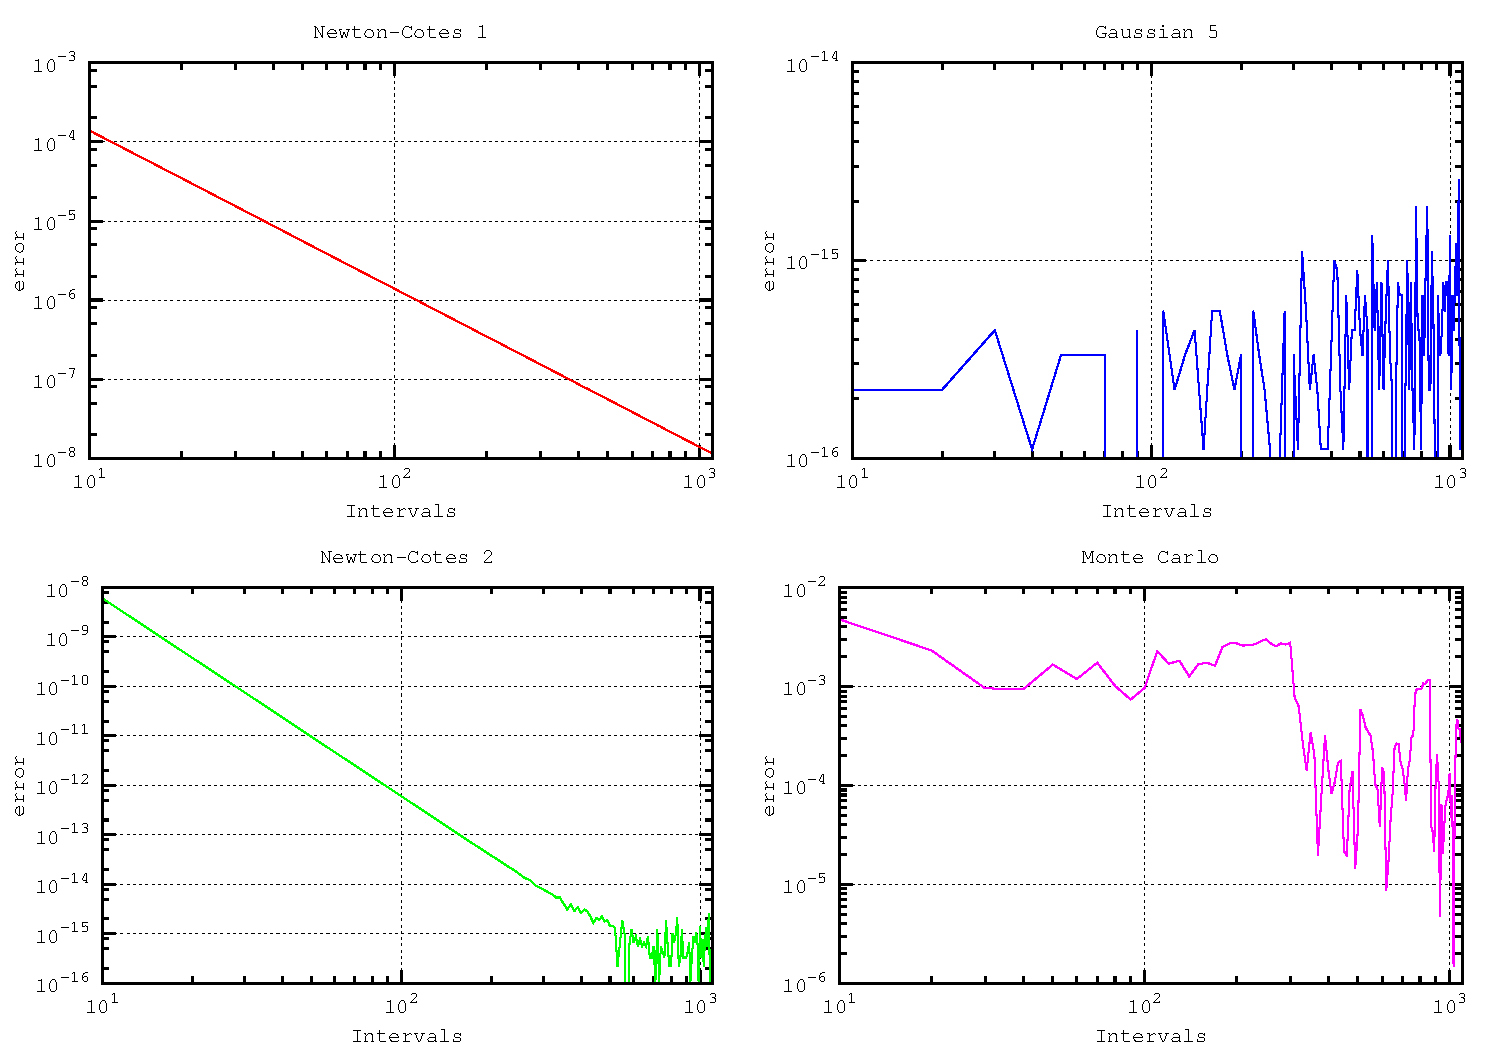
\includegraphics[width=\textwidth]{integral}
\caption{Errore calcolato}
\label{fig:integral}
\end{figure}

Come previsto, il metodo Monte Carlo risulta il più impreciso. con un errore che oscilla anche di due ordini di grandezza. Il Monte Carlo è infatti impiegato prevalentemente in quei casi in cui la mole di calcoli da svolgere è troppo grande per poter impiegare algoritmi di tipo deterministico.
Dei metodi di quadratura invece l'algoritmo di Gauss-Legendre di grado $5$ è il più preciso, con errori dell'ordine di $10^{-15}$ anche per $n$ piccolo. Al di sotto di $10^{-15}$ l'errore diventa instabile a causa della precisione finita del calcolatore. Infine la precisione delle formule di Newton Cotes è bassa per $n$ piccolo ma aumenta all'aumentare di $n$ e del grado dell'approssimazione.
